\documentclass[12pt,a4paper]{article}
        \usepackage{graphicx}
        \usepackage{geometry}
        \geometry{margin=2cm}
        \usepackage{helvet}
        \usepackage{xcolor}
        \usepackage{amsmath} % for bmatrix
        \setlength{\parindent}{0pt}  % No indentation globally
        \renewcommand{\familydefault}{\sfdefault}
        \usepackage[german]{babel}% for glqq / grqq

        \begin{document}\begin{center}
                \Huge \textbf{Cyclopentadiene} \\[1cm]
                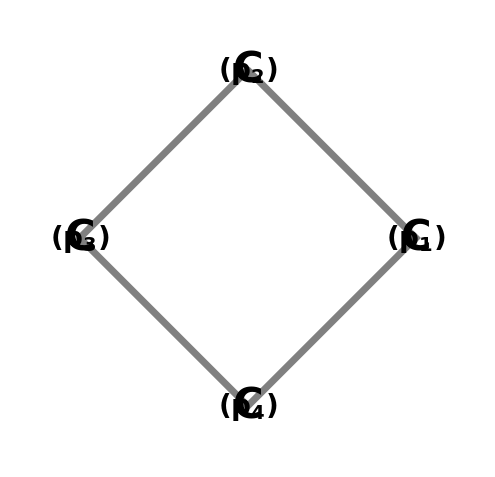
\includegraphics[width=0.5\textwidth]{cyclopentadiene} \\[0.5cm]
                \Large Point Group: \textbf{D4h}
            \end{center}\newpage\section*{p orbitals}
Symmetry behavior of the p-orbitals:
$$\mathsf{\Gamma}_{red} = \,4 E\;; \,-2 C'2\;; \,-4 \sigma h\;; \,2 \sigma v\;$$
$$\mathsf{\Gamma}_{irred} = \,1 Eg\;\oplus{}\,1 A2u\;\oplus{}\,1 B2u\;$$


\begin{itemize}
\item SALC of Eg: \quad $\frac{\sqrt{2} \left(\text{p}_{1} - \text{p}_{3}\right)}{2}$
\item SALC of A2u: \quad $\frac{\text{p}_{1}}{2} + \frac{\text{p}_{2}}{2} + \frac{\text{p}_{3}}{2} + \frac{\text{p}_{4}}{2}$
\item SALC of B2u: \quad $\frac{\text{p}_{1}}{2} - \frac{\text{p}_{2}}{2} + \frac{\text{p}_{3}}{2} - \frac{\text{p}_{4}}{2}$
\item SALC of Eg: \quad $\frac{\sqrt{2} \left(\text{p}_{2} - \text{p}_{4}\right)}{2}$
\end{itemize}
Put together these SALCs form the following Hamilton matrices:
     $$ H_{Eg}= \begin{pmatrix}\tilde{\alpha} & 0\\0 & \tilde{\alpha}\end{pmatrix}$$ 
     $$ H_{A2u}= \begin{pmatrix}\tilde{\alpha} + 2 \tilde{\beta}\end{pmatrix}$$ 
     $$ H_{B2u}= \begin{pmatrix}\tilde{\alpha} - 2 \tilde{\beta}\end{pmatrix}$$ 


Solving Hückels secular equations, that follow from these H, leads to:
\begin{itemize}
\item orbital of A2u with energy = 
                                $\tilde{\alpha} + 2 \tilde{\beta}$ \\
( 
$$
\begin{pmatrix}1\end{pmatrix} * \left(\begin{array}{c}\text{1. SALC in A2u}\end{array}\right) = \begin{pmatrix}1\end{pmatrix} * \begin{pmatrix}\frac{\text{p}_{1}}{2} + \frac{\text{p}_{2}}{2} + \frac{\text{p}_{3}}{2} + \frac{\text{p}_{4}}{2}\end{pmatrix} 
 $$ $$ = \frac{\text{p}_{1}}{2} + \frac{\text{p}_{2}}{2} + \frac{\text{p}_{3}}{2} + \frac{\text{p}_{4}}{2} 
 $$ 
 )

\item orbital of Eg with energy = 
                                $\tilde{\alpha}$ \\
( 
$$
\begin{pmatrix}1 & 0\end{pmatrix} * \left(\begin{array}{c}\text{1. SALC in Eg} \\ \text{2. SALC in Eg}\end{array}\right) = \begin{pmatrix}1 & 0\end{pmatrix} * \begin{pmatrix}\frac{\sqrt{2} \text{p}_{1}}{2} - \frac{\sqrt{2} \text{p}_{3}}{2}\\\frac{\sqrt{2} \text{p}_{2}}{2} - \frac{\sqrt{2} \text{p}_{4}}{2}\end{pmatrix} 
 $$ $$ = \frac{\sqrt{2} \left(\text{p}_{1} - \text{p}_{3}\right)}{2} 
 $$ 
 )

\item orbital of Eg with energy = 
                                $\tilde{\alpha}$ \\
( 
$$
\begin{pmatrix}0 & 1\end{pmatrix} * \left(\begin{array}{c}\text{1. SALC in Eg} \\ \text{2. SALC in Eg}\end{array}\right) = \begin{pmatrix}0 & 1\end{pmatrix} * \begin{pmatrix}\frac{\sqrt{2} \text{p}_{1}}{2} - \frac{\sqrt{2} \text{p}_{3}}{2}\\\frac{\sqrt{2} \text{p}_{2}}{2} - \frac{\sqrt{2} \text{p}_{4}}{2}\end{pmatrix} 
 $$ $$ = \frac{\sqrt{2} \left(\text{p}_{2} - \text{p}_{4}\right)}{2} 
 $$ 
 )

\item orbital of B2u with energy = 
                                $\tilde{\alpha} - 2 \tilde{\beta}$ \\
( 
$$
\begin{pmatrix}1\end{pmatrix} * \left(\begin{array}{c}\text{1. SALC in B2u}\end{array}\right) = \begin{pmatrix}1\end{pmatrix} * \begin{pmatrix}\frac{\text{p}_{1}}{2} - \frac{\text{p}_{2}}{2} + \frac{\text{p}_{3}}{2} - \frac{\text{p}_{4}}{2}\end{pmatrix} 
 $$ $$ = \frac{\text{p}_{1}}{2} - \frac{\text{p}_{2}}{2} + \frac{\text{p}_{3}}{2} - \frac{\text{p}_{4}}{2} 
 $$ 
 )

\end{itemize}



\newpage \section*{s orbitals}
Symmetry behavior of the s-orbitals:
$$\mathsf{\Gamma}_{red} = \,4 E\;; \,2 C'2\;; \,4 \sigma h\;; \,2 \sigma v\;$$
$$\mathsf{\Gamma}_{irred} = \,1 A1g\;\oplus{}\,1 B1g\;\oplus{}\,1 Eu\;$$


\begin{itemize}
\item SALC of A1g: \quad $\frac{\text{s}_{1}}{2} + \frac{\text{s}_{2}}{2} + \frac{\text{s}_{3}}{2} + \frac{\text{s}_{4}}{2}$
\item SALC of B1g: \quad $\frac{\text{s}_{1}}{2} - \frac{\text{s}_{2}}{2} + \frac{\text{s}_{3}}{2} - \frac{\text{s}_{4}}{2}$
\item SALC of Eu: \quad $\frac{\sqrt{2} \left(\text{s}_{1} - \text{s}_{3}\right)}{2}$
\item SALC of Eu: \quad $\frac{\sqrt{2} \left(\text{s}_{2} - \text{s}_{4}\right)}{2}$
\end{itemize}
Put together these SALCs form the following Hamilton matrices:
     $$ H_{A1g}= \begin{pmatrix}\tilde{\alpha}_{s} + 2 \tilde{\beta}_{s}\end{pmatrix}$$ 
     $$ H_{B1g}= \begin{pmatrix}\tilde{\alpha}_{s} - 2 \tilde{\beta}_{s}\end{pmatrix}$$ 
     $$ H_{Eu}= \begin{pmatrix}\tilde{\alpha}_{s} & 0\\0 & \tilde{\alpha}_{s}\end{pmatrix}$$ 


Solving Hückels secular equations, that follow from these H, leads to:
\begin{itemize}
\item orbital of A1g with energy = 
                                $\tilde{\alpha}_{s} + 2 \tilde{\beta}_{s}$ \\
( 
$$
\begin{pmatrix}1\end{pmatrix} * \left(\begin{array}{c}\text{1. SALC in A1g}\end{array}\right) = \begin{pmatrix}1\end{pmatrix} * \begin{pmatrix}\frac{\text{s}_{1}}{2} + \frac{\text{s}_{2}}{2} + \frac{\text{s}_{3}}{2} + \frac{\text{s}_{4}}{2}\end{pmatrix} 
 $$ $$ = \frac{\text{s}_{1}}{2} + \frac{\text{s}_{2}}{2} + \frac{\text{s}_{3}}{2} + \frac{\text{s}_{4}}{2} 
 $$ 
 )

\item orbital of Eu with energy = 
                                $\tilde{\alpha}_{s}$ \\
( 
$$
\begin{pmatrix}1 & 0\end{pmatrix} * \left(\begin{array}{c}\text{1. SALC in Eu} \\ \text{2. SALC in Eu}\end{array}\right) = \begin{pmatrix}1 & 0\end{pmatrix} * \begin{pmatrix}\frac{\sqrt{2} \text{s}_{1}}{2} - \frac{\sqrt{2} \text{s}_{3}}{2}\\\frac{\sqrt{2} \text{s}_{2}}{2} - \frac{\sqrt{2} \text{s}_{4}}{2}\end{pmatrix} 
 $$ $$ = \frac{\sqrt{2} \left(\text{s}_{1} - \text{s}_{3}\right)}{2} 
 $$ 
 )

\item orbital of Eu with energy = 
                                $\tilde{\alpha}_{s}$ \\
( 
$$
\begin{pmatrix}0 & 1\end{pmatrix} * \left(\begin{array}{c}\text{1. SALC in Eu} \\ \text{2. SALC in Eu}\end{array}\right) = \begin{pmatrix}0 & 1\end{pmatrix} * \begin{pmatrix}\frac{\sqrt{2} \text{s}_{1}}{2} - \frac{\sqrt{2} \text{s}_{3}}{2}\\\frac{\sqrt{2} \text{s}_{2}}{2} - \frac{\sqrt{2} \text{s}_{4}}{2}\end{pmatrix} 
 $$ $$ = \frac{\sqrt{2} \left(\text{s}_{2} - \text{s}_{4}\right)}{2} 
 $$ 
 )

\item orbital of B1g with energy = 
                                $\tilde{\alpha}_{s} - 2 \tilde{\beta}_{s}$ \\
( 
$$
\begin{pmatrix}1\end{pmatrix} * \left(\begin{array}{c}\text{1. SALC in B1g}\end{array}\right) = \begin{pmatrix}1\end{pmatrix} * \begin{pmatrix}\frac{\text{s}_{1}}{2} - \frac{\text{s}_{2}}{2} + \frac{\text{s}_{3}}{2} - \frac{\text{s}_{4}}{2}\end{pmatrix} 
 $$ $$ = \frac{\text{s}_{1}}{2} - \frac{\text{s}_{2}}{2} + \frac{\text{s}_{3}}{2} - \frac{\text{s}_{4}}{2} 
 $$ 
 )

\end{itemize}



\newpage \section*{Transitions from p orbitals into s orbitals}\subsection*{State with Occupation (2, 2, 0, 0) (0 unpaired electrons, mult 1.0)}
        \noindent\textbf{Transition from $\psi_{2}$ into $\psi_{\text{s}_{2}}$:}
        \begin{itemize}
            \item $- (2, 2, 0, 0), (0, 0, 0, 0) \rightarrow (2, 1, 0, 0), (0, 1, 0, 0)$
        
            \item $\psi_{2}:$ linear combination = $\sqrt{2} \left(\text{p}_{1} - \text{p}_{3}\right)$, \
            energy = $\tilde{\alpha}$
            
            \item $\eta_{2}:$ linear combination = $\sqrt{2} \left(\text{s}_{1} - \text{s}_{3}\right)$, \
            energy = $\tilde{\alpha}_{s}$
            
                \item $\Delta$ Energy: $- \tilde{\alpha} + \tilde{\alpha}_{s}$
                \item Energy of State before Excitation: $4 \tilde{\alpha} + 4 \tilde{\beta}$
                \item Energy of State after Excitation: $3 \tilde{\alpha} + \tilde{\alpha}_{s} + 4 \tilde{\beta}$
                \item Energy between Average Energies of $\psi$-/$\eta$-orbitals: $- \tilde{\alpha} + \tilde{\alpha}_{s}$
            
            \item dipole transition moment: $\tilde{\delta}$
        
        \end{itemize}
        
\subsection*{State with Occupation (2, 1, 1, 0) (2 unpaired electrons, mult 3.0)}
        \noindent\textbf{Transition from $\psi_{2}$ into $\psi_{\text{s}_{2}}$:}
        \begin{itemize}
            \item $- (2, 1, 1, 0), (0, 0, 0, 0) \rightarrow (2, 0, 1, 0), (0, 1, 0, 0)$
        
            \item $\psi_{2}:$ linear combination = $\sqrt{2} \left(\text{p}_{1} - \text{p}_{3}\right)$, \
            energy = $\tilde{\alpha}$
            
            \item $\eta_{2}:$ linear combination = $\sqrt{2} \left(\text{s}_{1} - \text{s}_{3}\right)$, \
            energy = $\tilde{\alpha}_{s}$
            
                \item $\Delta$ Energy: $- \tilde{\alpha} + \tilde{\alpha}_{s}$
                \item Energy of State before Excitation: $4 \tilde{\alpha} + 4 \tilde{\beta}$
                \item Energy of State after Excitation: $3 \tilde{\alpha} + \tilde{\alpha}_{s} + 4 \tilde{\beta}$
                \item Energy between Average Energies of $\psi$-/$\eta$-orbitals: $- \tilde{\alpha} + \tilde{\alpha}_{s}$
            
            \item dipole transition moment: $\tilde{\delta}$
        
        \end{itemize}
        

        \noindent\textbf{Transition from $\psi_{3}$ into $\psi_{\text{s}_{3}}$:}
        \begin{itemize}
            \item $- (2, 1, 1, 0), (0, 0, 0, 0) \rightarrow (2, 1, 0, 0), (0, 0, 1, 0)$
        
            \item $\psi_{3}:$ linear combination = $0$, \
            energy = $\tilde{\alpha}$
            
            \item $\eta_{3}:$ linear combination = $0$, \
            energy = $\tilde{\alpha}_{s}$
            
                \item $\Delta$ Energy: $- \tilde{\alpha} + \tilde{\alpha}_{s}$
                \item Energy of State before Excitation: $4 \tilde{\alpha} + 4 \tilde{\beta}$
                \item Energy of State after Excitation: $3 \tilde{\alpha} + \tilde{\alpha}_{s} + 4 \tilde{\beta}$
                \item Energy between Average Energies of $\psi$-/$\eta$-orbitals: $- \tilde{\alpha} + \tilde{\alpha}_{s}$
            
            \item dipole transition moment: $\tilde{\delta}$
        
        \end{itemize}
        
 -  AND 
\newpage \section*{Dispersion energies following from the transitions}

\begin{enumerate}
 \item State: A = (2, 1, 1, 0) $\leftrightarrow$ B = (2, 1, 1, 0) 
$$E_{dispersion} =- \frac{8 \tilde{\delta}^{4}}{r^{6} \left(\tilde{\alpha} - \tilde{\alpha}_{s}\right)}$$
\end{enumerate}
Ground-State:

A =[2, 2, 0, 0]$\leftrightarrow$ B =[2, 2, 0, 0]
$$E_{dispersion} =
- \frac{8 \tilde{\delta}^{4}}{r^{6} \left(\tilde{\alpha} - \tilde{\alpha}_{s}\right)}$$


\end{document}